\documentclass[
 reprint,
 amsmath,amssymb,
 aps,
]{revtex4-1}

\usepackage{graphicx}
\usepackage{dcolumn}
\usepackage{bm}

\begin{document}

\preprint{APS/123-QED}

\title{Percolaci\'on de nodos en redes cuadradas 2d}
\author{Felipe Gonzalez}
\affiliation{
 Departamento de F\'\i sica, Facultad de Ciencias Exactas y Naturales, Universidad de Buenos Aires,\\
 Pabell\'on I, Ciudad Universitaria, 1428 Buenos Aires, Argentina.
}

\date{\today}

\begin{abstract}
A partir de estudios computacionales sobre la percolaci\'on de redes de nodos de varios tama\~nos se logr\'o determinar el comportamiento cr\'\i tico del sistema. Se determinaron tanto los exponentes cr\'\i ticos como la probabilidad cr\'\i tica de la red bidimensional con concordancia a lo predicho te\'oricamente. Se extrapol\'o para una red infinita una probabilidad cr\'\i tica tal que existe un cluster percolante para cualquier probabilidad mayor a ella de $p_c(\infty) = (0.593 \pm 0.002)$.

\end{abstract}

\maketitle

\section{Introducci\'on}

Los primeros estudios de percolacion los realizon Flory y Stockmayer alrededor de los a\~nos 40, durante la segunda guerra mundial. Usualmente los comienzos de la teor\'\i a se atribuyen al trabajo de Broadbent y Hammersley en el a\~no 1957, introduciendo un tratamiento mat\'ematico, probabil\'\i stico y geom\'etrico del mismo. A pesar de esto, la teor\'\i a de percolaci\'on enfocada a los exponentes cr\'\i ticos, comenz\'o a desarrollarse en la d\'ecada del 70, a partir del trabajo de Essam y Gwilym, que desataron una avalancha de publicaciones en esa \'epoca. En resumidas palabras, la teor\'\i a de percolaci\'on tiene como objetivo, estudiar y resolver de manera simplificada, aunque no de manera exacta, transiciones de fase, a partir de un modelo basado en redes de nodos que pueden estar ocupados o no.

El modelo trabaja con diversas redes, desde redes unidimensionales hasta redes de dimensi\'on infinita, donde cada nodo o sitio de la red tendr\'a una cierta probabilidad $p$ de estar ocupado o desocupado, y la misma ser\'a independiente de la situaci\'on del nodo vecino. Grupos de vecinos inmediatos ocupados forman agrupaciones, que comunmente se los conoce como clusters. Uno de los objetivos de este modelo es estudiar el comportamiento del sistema en el rango de probabilidades cercanas a una probabilidad cr\'\i tica. La misma se corresponde con la aparici\'on del cluster percolante (que atraviesa toda la red de arriba a abajo) en la red utilizada.


\section{El modelo}

\subsection{Transici\'on de fase}

Cuando se var\'\i a la probabilidad de ocupaci\'on de los nodos de una red, se observa que existe un valor de probabilidad a partir del cual aparece un cluster percolante en la red que se est\'a observando. Esto refleja una transici\'on de fase, donde el par\'ametro de orden de la misma es la intensidad del cluster percolante (definido como el n\'umero de nodos que son parte del cluster percolante en relaci\'on al total de nodos de la red), el cual es nulo para probabilidades menores o iguales que la cr\'\i tica, para luego crecer con una ley de potencias a medida que se aumenta la probabilidad. Uno de los objetivos del estudio de las transiciones de fase es observar el comportamiento de diversas magnitudes asociadas al sistema en un entorno cercano al punto de la transici\'on de fase. El comportamiento de estas magnitudes es diferente en cada caso: ciertas magnitudes presentan discontinuidades, algunas divergen, y otras comienzan a ser distintas de cero. Para explicar este comportamiento, es necesario recurrir a los exponentes cr\'\i ıticos (el comportamiento de las magnitudes puede describirse como leyes de potencia), que son particulares del sistema que se est\'e analizando. En la pr\'oxima secci\'on se ampliar\'a el tema para sistemas percolantes en redes bidimensionales.

\subsection{\label{critical}Leyes de potencia y exponentes cr\'\i ticos}

Los exponentes cr\'\i ticos, describen el comportamiento de ciertas magnitudes cerca de una transici\'on de fase. Como se mencion\'o anteriormente, en percolaci\'on, la transici\'on resulta en la aparici\'on de un cluster infinito. Estos exponentes son universales, en el sentido que dependen solo del modelo de percolaci\'on utilizado y de la dimensi\'on espacial. La Tabla~\ref{valores_teoricos} resume las principales leyes de potencia obtenidas en la literatura para redes percolantes.

\begin{table}[h]
\caption{\label{valores_teoricos}
Valores te\'oricos hallados en la literatura.
}
\begin{ruledtabular}
\begin{tabular}{lll}
\\[-5pt]
 S\'\i mbolo     & Ley                        & Valor                          \\
\hline
$d$             &   ---                         & $d=2$                        \\
$D$             & $M\sim L^{D}$                 & $D=91/48$                    \\
$\nu$           & $\xi\sim|p-p_c|^{-\nu}$       & $\nu=4/3$                    \\
$\tau$          & $n(p_c)\sim s^{-\tau}$        & $\tau=1+d/D$                 \\
$\sigma$        & $z=s^\sigma(p-p_c)$           & $\sigma=(\nu D)^{-1}$        \\
$\alpha$        & $m_0(p)\sim|p-p_c|^{2-\alpha}$& $\alpha=2-(\tau-1)/\sigma$   \\
$\beta$         & $m_1(p)\sim(p-p_c)^\beta$     & $\beta=\nu(d-D)$             \\
$\gamma$        & $m_2(p)\sim|p-p_c|^{-\gamma}$ & $\gamma=(3-\tau)/\sigma$     \\
\end{tabular}
\end{ruledtabular}
\end{table}

La intensidad del cluster percolante est\'a dada por la relaci\'on $P \propto |p - p_c|^\beta$ para $p$ mayor a $p_c$, y es nula en otro caso. El n\'umero de clusters de tama\~no $s$ que aparecen a probabilidad $p$ est\'a dado por la expresi\'on $n_s(p) = q_o s^{-\tau}$. Otra relaci\'on importante para obtener el exponente cr\'\i tico $\gamma$, es el momento de orden 2, cuya ecuaci\'on es la que sigue:

\begin{equation}\label{momento_2_gamma}
    m_2(p) = \sum_s s^2n_s(p) \simeq | p - p_c |^{-\gamma}
\end{equation}


Como se detallar\'a con mayor detalle en la pr\'oxima secci\'on, para obtener el exponente $\tau$, es necesario detallar la dependecia del factor $q_0$ con el exponente cr\'\i tico $\tau$. En este trabajo, obtendremos inicialmente una primera estimaci\'on del exponente cr\'\i tico $\tau$, sin dar la dependencia de $q_0$, y luego, desarrollando otro m\'etodo, se obtendr\'a una mejor estimaci\'on del mismo. Otro punto importante a se\~nalar es la dependecia de la masa del cluster percolante respecto del tama\~no de la red en funci\'on de la probabilidad. En el punto cr\'\i tico, la masa del cluster infinito es proporcional al factor $L^D$ del tama\~no de la red. $D$ se conoce como dimensi\'on fractal. En probabilidades por encima de la cr\'\i tica, la masa es en cambio propocional al tama\~no de la red $L$ elevado a la dimensi\'on de la red $d$; como en este trabajo se utilizaron solo redes bidimen- sionales, se tiene que $d = 2$. Esto se puede ver resumido en la ecuaci\'on \ref{masa_eqn}.

\begin{equation}\label{masa_eqn}
    M(L) = \left \{ \begin{matrix} L^d \; \text{si } p > p_c \\  L^D \; \text{si } p < p_c \end{matrix} \right .
\end{equation}

Con el momento de orden 1, $m_1(p)$, se puede obtener el exponente cr\'\i tico $\beta$, que a su vez se puede obtener a partir de $\nu$ y $D$. Este momento se calcula a partir de la intensidad del cluster percolante. El momento de orden 2, $m_2(p)$ nos da informaci\'on sobre el exponente $\gamma$.

\subsection{\label{scaling}Efectos de red finita}

Cuando se busca resolver num\'ericamente problemas de percolaci\'on, se tiene acceso a una ventana finita de la red infinita que se propone te\'oricamente. Cerca de la probabilidad cr\'\i tica, magnitudes que presentan cambios abruptos en las redes infinitas, lo hacen de manera suave para las finitas. En resumen, el comportamiento de una red de tama\~no finito se aparta del correspondiente para tama\~no infinito. En cambio, en el punto de transici\'on se encuentra que el sistema est\'a libre de escalas y se pueden utilizar la leyes de exponentes cr\'\i ticos.
La ecuaci\'on \ref{eqn_1} expresa la relaci\'on funcional entre el n\'umero de cluster de tama\~no $s$, y el valor de $s$, utilizando una cierta funci\'on $f(z)$, la cual es determinada por m\'etodos computacionales. La misma deber\'a satisfacer las restricciones f\'\i sicas implicadas. Debido a que en la probabilidad cr\'\i tica se espera una ley de potencias sobre $s$, es necesario que $f(0)=1$. Adem\'as, dado que para un $s$ existe una cierta probabilidad que maximiza el n\'umero de clusters de ese tama\~no, eso conlleva a que la funci\'on $f(z)$ presente un \'unico m\'aximo. La funci\'on tambien debe anularse cuando $z$ tiende a $\pm \infty$.

\begin{equation}
n_s(p) = q_0\,s^{-\tau}\,f(z)\ \ \ \ ,\ \ \ \ z=s^\sigma(p-p_c)\label{eqn_1}
\end{equation}

\subsection{\label{renorm}Renormalizaci\'on}

Es posible adem\'as, explotar el hecho de que cerca de la transici\'on de fase de muestra libre de escalas. Si se reescalea el sistema, deben seguir siendo validas las leyes de potencias anteriores. Esto refleja el hecho que la probabilidad cr\'\i tica es un punto fijo respecto de la transformaci\'on. Dada una probabilidad, si la misma no coincide con la cr\'\i tica y el sistema es reescaleado, la probabilidad tender\'a a dos atractores, el $0$ y el $1$, dependiendo de donde se tomo la probabilidad inicial. Esto implica que al renormalizar, me alejo del punto cr\'\i tico. En cambio, si se toma como inicial la cr\'\i tica, el sistema se mantiene igual al ser reescaleado, se reconstruye a si mismo. Esto se debe a que la distancia de correlaci\'on, infinita en $p_c$, seguir\'a siendo infinita, puesto que la renormalizacion siempre ser\'a sobre un valor finito. Al manterse infinita, implicar\'a siempre estar en $p_c$. Cabe destacar que la renormalizaci\'on de celda peque\~na solo es v\'alida para redes triangulares y redes bidimensionales. Por otro lado, es importante se\~nalar que hay que elegir el criterio de normalizaci\'on que mas se asemeje a la situaci\'on f\'\i sica del problema.

\section{\label{simulations}Simulaciones num\'ericas}

Se estudiaron redes cuadradas de tama\~no $L=4, 16, 32, 64, 128$ por medio del algoritmo de clasificaci\'on de Hoshen-Kopelman \cite{Kopelman}. De las mismas se obtuvo la probabilidad cr\'\i tica por diferentes m\'etodos, uno de ellos promediando varios resultados obtenidos para redes generadas a partir de diferentes semillas de n\'umeros aleatorios, de los cuales se obtuvo la dispersi\'on y se calcul\'o la probabilidad cr\'\i tica correspondiente a la red infinita.
Se determinaron los exponentes cr\'\i ticos a partir de las leyes dadas para cada uno, estudiando tama\~no de clusters, distribuci\'on de los mismos en funci\'on de la probabilidad, entre otras cosas.
Se determina la dimensi\'on fractal $D$ a partir de la masa del cluster percolante, que se calcula como el numero de nodos pertenecientes al mismo, y observando su dependencia con $L$.
A partir del c\'alculo de la intensidad del cluster percolante se puede obtener el exponente cr\'\i tico $\beta$, modelando su comportamiento cerca de $p_c$ como una ley de potencias.
Se verifica la hip\'otesis de scaling encontrando la forma funcional de la funci\'on de scaleo $f(z)$. A partir de la misma, se puede calcular el valor de $\tau$ siguiendo la correspondiente ley de potencias ya mencionada.
Finalmente, para obtener el exponente $\gamma$ se realiza un proceso de gamma-matching, donde se calcula el momento de segundo orden y se observa su comportamiento en funci\'on de $p$.


\begin{equation}
M(L)=L^D\,m\bigg(\displaystyle\frac{L}{\xi}\bigg)\sim\left\{\begin{array}{lll}
             L^D       & \textrm{si} & L<\xi \\
             L^d       & \textrm{si} & L\gg\xi \\
            \end{array}\right.\label{eqn_2}
\end{equation}


\section{\label{results}Resultados}

\subsection{\label{p_c} Determinaci\'on de $p_c(\infty)$, y $\tau$}

Se usaron distintos m\'etodos para la determinaci\'on num\'erica del punto cr\'\i tico, siendo estos la b\'usqueda de $p_\mathrm{medio}$ y b\'usqueda de $p_\mathrm{mediana}$. Es importante se\~nalar que la probabilidad cr\'\i tica corresponder\'a a la ventana de la red infinita a la que se tiene acceso. Por ello, es que para cada tama\~no de red obtendremos diferentes probabilidades cr\'\i ticas, las cuales ir\'an convergiendo a la probabilidad cr\'\i tica infinita a medida que se aumente el tama\~no de la ventana que se est\'a observando.
Se comenz\'o un primer estudio de $p_{medio}$, con el fin de encontrar la probabilidad cr\'\i tica. Dado un tama\~no de red fijo, se poblaron nodos de la red aleatoriamente a partir de una semilla de n\'umeros aleatorios y se verific\'o si la red percolaba o no. En caso afirmativo, se disminuye la probabilidad rest\'andole $\frac{1}{2^n}$ (para el en\'esimo paso) y se vuelve a poblar la red con la misma semilla y esta nueva probabilidad de ocupaci\'on de los nodos. En caso negativo, la probabilidad se aumenta en la misma cantidad que se rest\'o en el caso anterior y se realiza el mismo proceso de repoblaci\'on de la red. Esto se realiz\'o para los tama\~nos de red $4, 16, 32, 64$ y $128$, y se tom\'o la probabilidad cr\'itica como el valor de probabilidad de la \'ultima iteraci\'on en que el sistema percola, tomando como precisi\'on la m\'\i nima variaci\'on de probabilidad que se suma o resta, siendo esta $\frac{1}{2^{12}} \simeq 0.0002$. Se realiza el mismo proceso $27000$ veces, en pos de conseguir una muestra razonable para poder hacer estad\'\i stica.

Los resultados de este experimento se encuentran en la tabla \ref{tabla_p_c}.

\begin{table}[h]
\caption{\label{tabla_p_c} Valores de $p_c$ obtenidos para los distintos tama\~nos de red con metodo de $p_{medio}$}
\begin{ruledtabular}
\begin{tabular}{lll}
\\[-5pt]
 Tama\~no de red     & $p_c$\\
\hline
4   &  $(0.56 \pm 0.10)$ \\
16  &  $(0.588 \pm 0.044)$ \\
32  &  $(0.592 \pm 0.027)$ \\
64  &  $(0.593 \pm 0.017)$ \\
128 &  $(0.5926 \pm 0.0099)$ \\

\end{tabular}
\end{ruledtabular}
\end{table}

Como segundo m\'etodo de estimaci\'on de la probabilidad cr\'\i tica, se estudi\'o el promedio de veces que una red percola en funci\'on de la probabilidad de llenado. Se realiza un barrido sobre este par\'ametro para conseguir la funci\'on distribucion $F(p)$ del problema. Siendo que las redes estudiados son de tama\~no finito, fueron realizadas $27000$ mediciones por cada valor de probabilidad en pos de asegurar que el promedio de las realizaciones se corresponde a la verdadera estad\'\i stica del problema y reducir la susceptibilidad a \emph{outliers}. Se tom\'o como probabilidad cr\'\i tica el valor medio de la distribuci\'on de probabilidad $f(p)$.

Sobre las figuras \ref{F(p)} y \ref{f(p)} se pueden ver las funci\'on de distribucion y la distribuci\'on de probabilidad de percolaci\'on de la red en funci\'on de la probabilidad de llenado (respectivamente). Se puede ver como a medida que crece $L$, las distribuciones se acercan a la funci\'on de Heavyside y la delta de Dirac, como lo predice la teor\'\i a.

Tenemos as\'i una herramienta para extrapolar la probabilidad de percolaci\'on de una red infinita, siendo que podemos ver que el ancho de las campanas decrece de manera mon\'otona a medida que aumenta el tama\~no de la red. Se propone entonces realizar un ajuste lineal sobre la curva de $p_c(L)$ en funci\'on del ancho de las distribuciones de probabilidad. Esto se encuentra en la figura \ref{ajuste}. Se tiene que realizando este analisis, se llega a una $p_c(\infty) = (0.593 \pm 0.002)$, que es compatible con el valor te\'orico de $p_c_\text{teo}(\infty) = 0.5927$.

\begin{figure}[ht]
\begin{center}
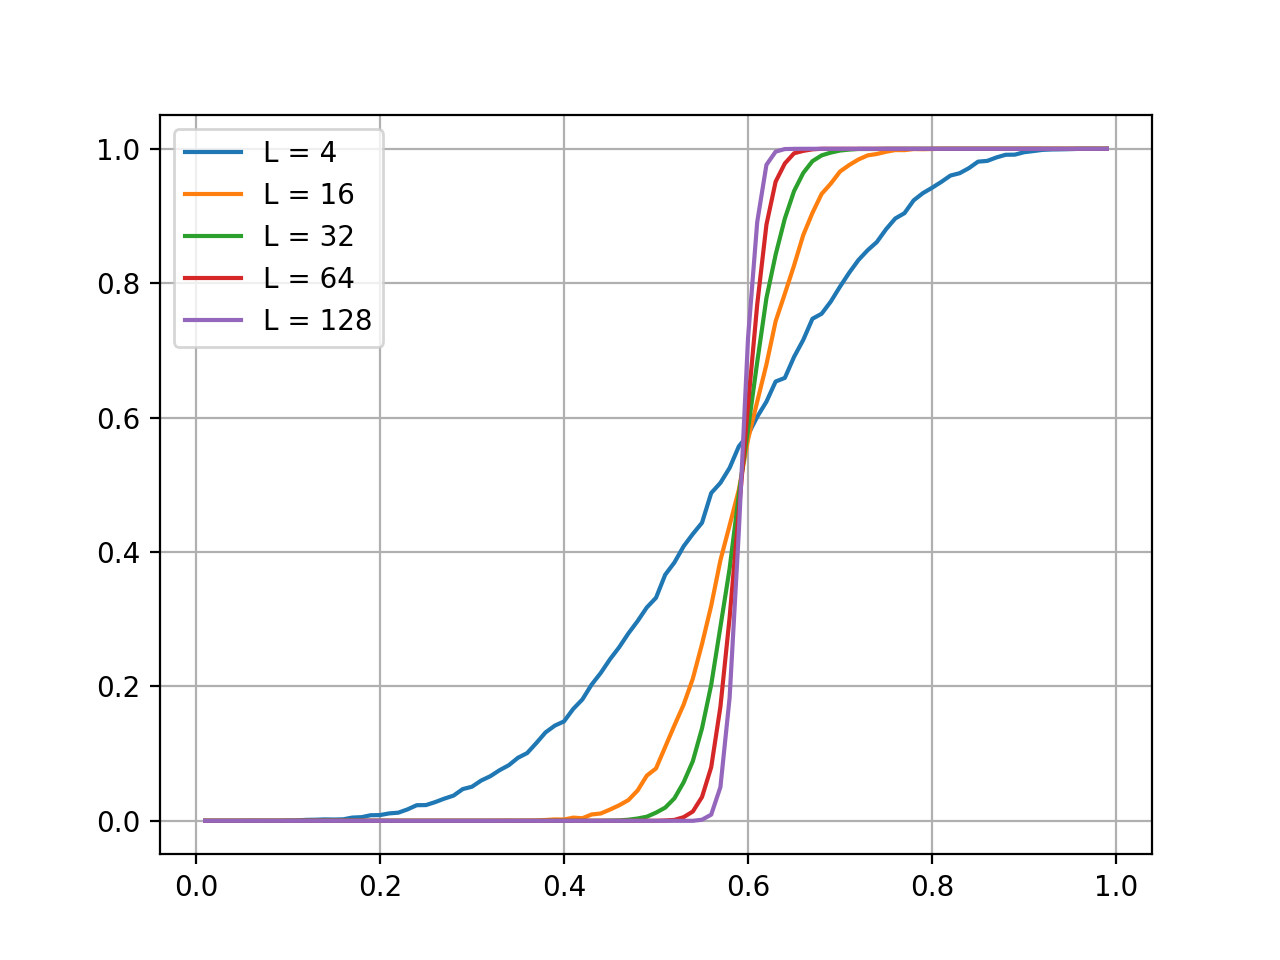
\includegraphics[scale=0.62]{../images/F(p).png} \\
\caption{Funcion distribucion $F(p)$ de la probabilidad de percolacion en funcion de la probabilidad de llenado de la red, para los distintos tama\~nos de red.}\label{F(p)}
\end{center}
\end{figure}

\begin{figure}[ht]
\begin{center}
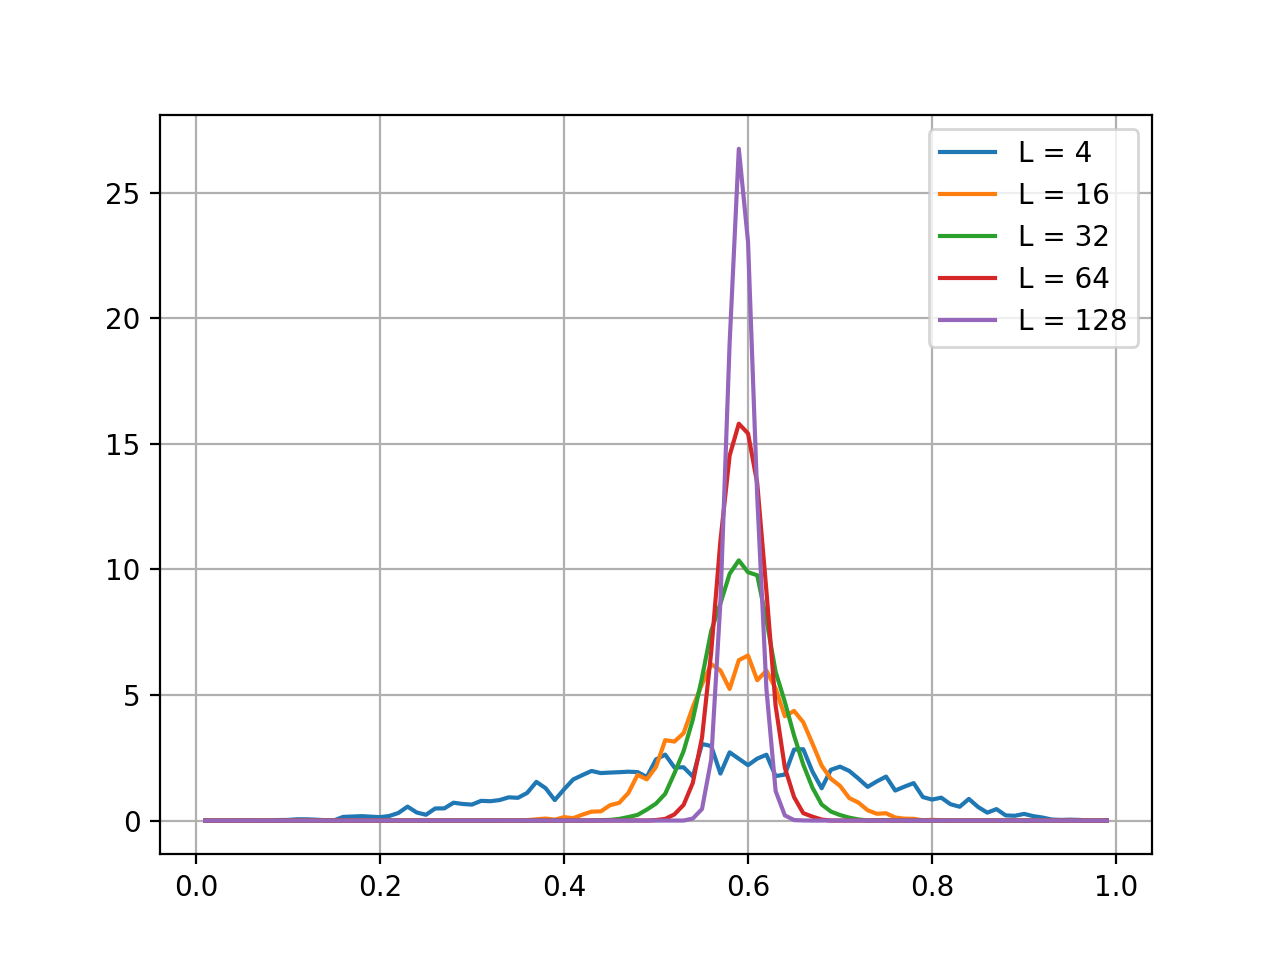
\includegraphics[scale=0.62]{../images/_f(p).png} \\
\caption{Distribuci\'on de probabilidad $f(p)$ de la probabilidad de percolaci\'on en funcion de la probabilidad de llenado de la red. Se puede ver como el momento de orden dos de las distribuciones se achica a medida que crece el tama\~no de la red de percolaci\'on, resultando en campanas mas finas.}\label{f(p)}
\end{center}
\end{figure}

\begin{figure}[ht]
\begin{center}
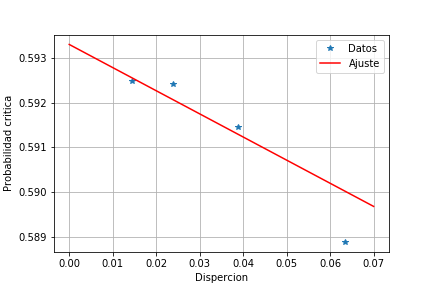
\includegraphics[scale=0.62]{../images/ajuste.png} \\
\caption{Ajuste lineal sobre la curva de la probabilidad cr\'\i tica en funci\'on de la dispersion de la medici\'on, $p_c(\infty) = (0.593 \pm 0.002)$}\label{ajuste}
\end{center}
\end{figure}

A partir de los valores de probabilidad cr\'\i tica obtenidos, se obtuvieron datos de tama\~nos de clusters en la red ($s$) y n\'umero de clusters con tama\~no $s$ ($n_s$), fijando la probabilidad en $p_c(L)$. Si se grafica $n_s$ vs $s$ en escala logar\'\i tmica, seg\'un la ley para el exponente cr\'\i tico $\tau$, se deber\'\i a observar un comportamiento lineal, cuya pendiente corresponde a este exponente cr\'\i tico. Esto se puede ver sobre la figura \ref{n_s_vs_s_ajuste}, donde se realiza un ajuste que resulta en un valor de $\tau = (1.809 \pm 0.002)$.
Tenemos que este valor esta por debajo del predicho te\'oricamente, y no cumple la restricci\'on de ser $>2$ (esto se debe a que se debe cumplir que $\tau = 1 + \frac{d}{D}$, con $D < d$). Esto se debe a que existe una dependencia entre la ordenada al or\'igen ($q_0$) y $\tau$ que no esta siendo tenida en cuenta, ya que se cumple que $q_0 = \frac{p_c}{\Chi(\tau - 1)}$. Teniendo esto en cuenta, se repite el ajuste y se llega un valor de $\tau = (2.103 \pm 0.004)$ (figura \ref{n_s_vs_s_ajuste_mejor}).
Vemos que este valor no esta lejos del valor te\'orico de $\tau_\text{teo} \simeq 2.05$.

\begin{figure}[ht]
\begin{center}
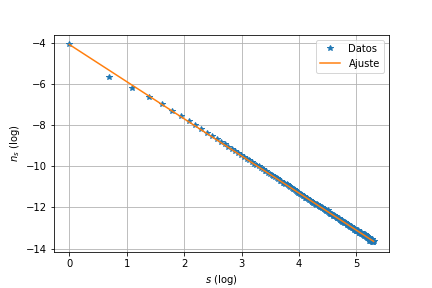
\includegraphics[scale=0.62]{../images/n_s_vs_s_ajuste.png} \\
\caption{Ajuste lineal sobre la curva del logaritmo de la distribuci\'on de fragmentos $n_s$ en funci\'on de el logaritmo del tama\~no del fragmento, sin restricci\'on sobre la ordenada al or\'igen. Se tiene que en estas condiciones el valor de $\tau = (1.809 \pm 0.002)$.}\label{n_s_vs_s_ajuste}
\end{center}
\end{figure}

\begin{figure}[ht]
\begin{center}
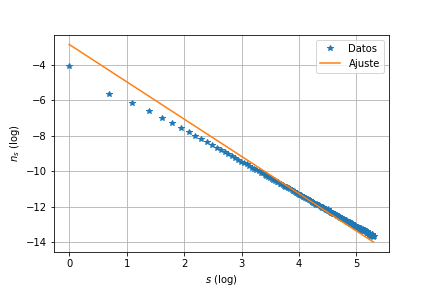
\includegraphics[scale=0.62]{../images/n_s_vs_s_ajuste_mejor.png} \\
\caption{Ajuste lineal sobre la curva del logaritmo de la distribuci\'on de fragmentos $n_s$ en funci\'on de el logaritmo del tama\~no del fragmento, restringiendo la ordenada al or\'igen a cumplir la relaci\'on correspondiente con el exponente, cuyo valor es $\tau = (2.103 \pm 0.004)$}\label{n_s_vs_s_ajuste_mejor}
\end{center}
\end{figure}


\subsection{\label{D} Determinaci\'on de la dimensi\'on fractal $D$ }

Seg\'un la Ec.~\ref{eqn_2} es posible hallar $D$ para un arreglo bidimensional, calculando la masa del cluster infinito en la probabilidad cr\'\i tica. Se poblaron redes de tama\~no $4, 16, 32, 64$ y $128$ con una probabilidad correspondiente a la probabilidad cr\'\i tica para cada tama\~no. Se realizaron $27000$ iteraciones para cada tama\~no, y se tomo la masa del cluster percolante como el promedio de la masa obtenido en cada iteracion. La figura \ref{masa_vs_L} muestra el logaritmo de la masa del cluster percolante en funci\'on del logaritmo del tamaño de la red. Tenemos que el ajuste nos deja un valor de $D = (1.84 \pm 0.01)$, un $5\%$ de diferencia respecto al valor te\'orico de $1.8958$.

\begin{figure}[ht]
\begin{center}
\includegraphics[scale=0.62]{../images/masa_vs_L.png} \\
\caption{Ajuste lineal sobre el logaritmo de la masa del cluster percolante sobre $p_c(L)$ en funcion del logaritmo de $L$. Esto nos da un valor de $D = (1.84 \pm 0.01)$.}\label{masa_vs_L}
\end{center}
\end{figure}

\subsection{\label{P} Obtenci\'on de $\beta$ a partir de la intensidad $P_\infty$}

A partir de la informaci\'on en el gr\'afico de $P_\infty(p)$ podemos hallar $\beta$, realizando un ajuste en un entorno cercano al punto cr\'\i tico. La figura \ref{masa_vs_p}, muestra la intensidad del cluster percolante en funci\'on de la probabilidad de llenado de la red. Se ilustran los resultados para $L = 128$.

\begin{figure}[ht]
\begin{center}
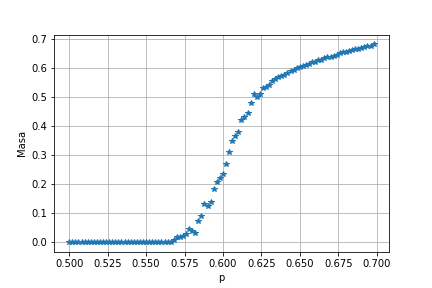
\includegraphics[scale=0.62]{../images/masa_vs_p.png} \\
\caption{Masa del cluster infinito en funcion de la probabilidad de llenado de la red. Vemos como se denota una transici\'on de fase, cuyo par\'ametro de orden es la intensidad del cluster percolante. $(L = 128)$}\label{masa_vs_p}
\end{center}
\end{figure}

Se observa que para probabilidades por debajo de la cr\'itica la intensidad del cluster percolante es nula, puesto que para esas probabilidades la red no percola. A partir del punto cr\'itico (valor al cual se espera, te\'oricamente, que sea el \'ultimo punto al cual la intensidad es nula) la intensidad comienza a crecer a medida que se aumenta la probabilidad. As\'\i, se tiene una transici\'on de fase de segundo orden (variable continua, derivada discontinua) cuyo par\'ametro de orden es la misma intensidad del cluster percolante. Se puede ver que la probabilidad en la cual la intensidad deja de ser nula es ligeramente menor que la esperada para una red infinita, que corresponde con la cr\'\i tica. Este corrimiento es uno de los efectos de trabajar con redes finitas, puesto que no se tiene acceso a la red infita. Debido a que la intensidad sigue una ley de potencias seg\'un el exponente cr\'\i tico, se calcula el mismo realizando un ajuste sobre la zona creciente de la curva, como se observa en la figura \ref{masa_vs_p_fit}.

\begin{figure}[ht]
\begin{center}
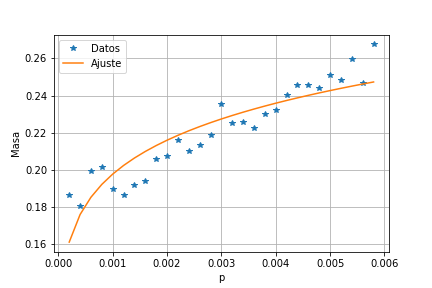
\includegraphics[scale=0.62]{../images/masa_vs_p_fit.png} \\
\caption{Ajuste de la relacion de potencia entre la intensidad del cluster infinito en funcion de la probabilidad de llenado de red. Esto corresponde a un valor de $\beta = (0.13 \pm 0.01)$.}\label{masa_vs_p_fit}
\end{center}
\end{figure}

Se obtuvo a partir del ajuste un valor de $\beta = (0.13 \pm 0.01)$ , el cual es compatible con el valor te\'orico, puesto que el mismo es $0,138$.

\subsection{\label{S} Espectro de fragmentos y verficaci\'on de la hip\'otesis de \emph{scaling} }

La hip\'otesis de \emph{scaling} se presenta en la Ec.~\ref{eqn_1} en donde se observa que para distintos valores de $s$ y $p-p_c$, el espectro de fragmentos debe colapsar en una \'unica curva $f(z)=n_s(p)/n_s(p_c)$, donde $z=s^\sigma(p-p_c)$. En consecuencia, verificamos la hip\'otesis de scaling graficando $f(z)$ y determinando el punto $f_{max} = f(z_{max})$, lo cual se puede observar en la figura \ref{f_vs_z} para varios valores de $s$. Este valor se corresponde con una probabilidad $p_{max}$ para cada tama\~no de $s$ fijo. La ley de exponente $\sigma$ sera entonces la siguiente:

\begin{equation}
\ln(p_\mathrm{max}-p_c)=-\sigma\,\ln(s)+\ln(z_\mathrm{max})+C\label{sigma}.
\end{equation}

\begin{figure}[ht]
\begin{center}
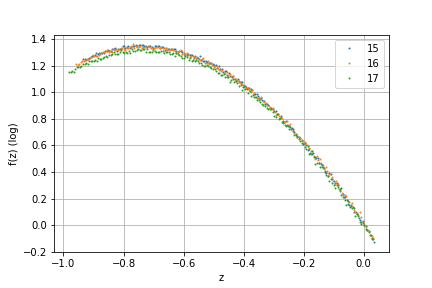
\includegraphics[scale=0.62]{../images/f_vs_z.png} \\
\caption{Logaritmo de la funci\'on de scaling en funcion de z para valores de $s$ desde $15$ a $17$.}\label{f_vs_z}
\end{center}
\end{figure}

Para obtener este exponente entonces se extraen los $p_{max}$ que cumplen maximizar la funci\'on $f(z)$ y se realiza un ajuste lineal sobre la curva que describe la ecuacion \ref{sigma}. Esto se puede ver en la figura \ref{eps_vs_s_ajuste}. Tenemos que la pendiente del ajuste corresponde a $\sigma = (0.40 \pm 0.02)$, que es indistinguible del valor te\'orico $\sigma_{teo} = 0.39$.

\begin{figure}[ht]
\begin{center}
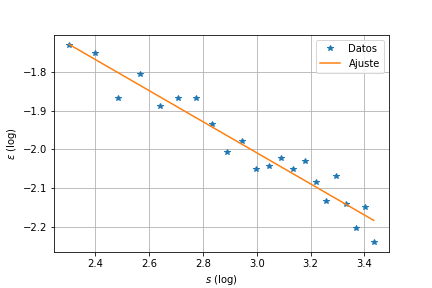
\includegraphics[scale=0.62]{../images/eps_vs_s_ajuste.png} \\
\caption{Ajuste sobre la curva del logaritmo de $\epsilon_\text{max}$ en funci\'on de el tama\~no de fragmento $s$. Corresponde a un $\sigma = (0.40 \pm 0.02)$.}\label{eps_vs_s_ajuste}
\end{center}
\end{figure}

Adem\'as, se calculo el exponente $\gamma$, a traves del momento de orden 2 de la red, utilizando la relacion descripta en la ecuaci\'on \ref{momento_2_gamma}. Para esto se realizo un barrido de probabilidad de llenado de red en el rango de $0.5 \leq p < 0.7$ con paso de $0.01$, promediando $10000$ iteraciones para cada probabilidad. Cabe destacar que se tuvo especial cuidado para remover el cluster percolante, asi asegurandose estar sumando solo los t\'erminos v\'alidos.

Tenemos que el momento de orden 2 de la distribucion de fragmentos se encuentra en la figura \ref{m_2_vs_epsilon}. Se puede ver que es completamente as\'imetrica, lo que lleva a proponer algun tipo de medici\'on que tenga en cuenta ambos lados de la funci\'on para obtener una mejor medida del exponente. Se comienza proponiendo un $\gamma$-matching, que consiste en tomar pendientes de ambos lados de la curva y en escala logaritmica en funci\'on del m\'inimo apartamiento de epsilon para cada lado, y tomar el $\gamma$ verdadero como la intersecci\'on de ambas mediciones.
Sin embargo tenemos que, como lo muestra la figura \ref{gamma_vs_epsilon}, estas 2 curvas no solo no se tocan sino que la distancia entre ellas crece a medida que crece el apartamiento, por lo que el an\'alisis no es posible.

\begin{figure}[ht]
\begin{center}
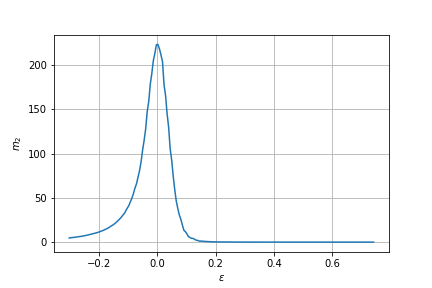
\includegraphics[scale=0.62]{../images/m_2_vs_epsilon.png} \\
\caption{Momento de \'orden 2 de la distribuci\'on de fragmentos en funcion de $\epsilon$.}\label{m_2_vs_epsilon}
\end{center}
\end{figure}

\begin{figure}[ht]
\begin{center}
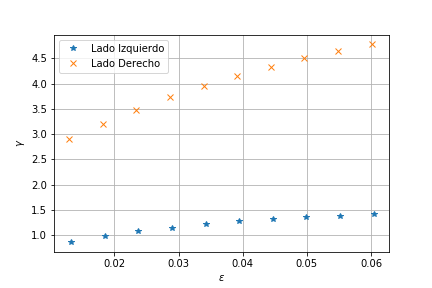
\includegraphics[scale=0.62]{../images/gamma_vs_epsilon.png} \\
\caption{Ajustes de $\gama$ en funci\'on del m\'inimo $\epsilon$ tomado para el ajuste, para ambos lados de $m_2$. Vemos que no solo las curvas no se intersecan, sino que tienden a alejarse.}\label{gamma_vs_epsilon}
\end{center}
\end{figure}

\begin{figure}[ht]
\begin{center}
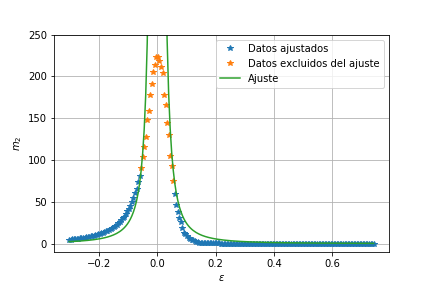
\includegraphics[scale=0.62]{../images/m_2_vs_epsilon_ajuste.png} \\
\caption{Ajuste no lineal sobre el momento de \'orden 2 de la distribuci\'on de fragmentos en funci\'on de $\epsilon$. Tenemos que esto corresponde a un $\gamma = (2.1 \pm 0.1)$.}\label{m_2_vs_epsilon_ajuste}
\end{center}
\end{figure}

En vez, se propone hacer un ajuste no lineal sobre la curva, excluyendo los puntos muy cercanos al punto cr\'itico para los cuales las mediciones fallan, siendo que es donde el momento deber\'ia diverger. Esto se puede ver en la figura \ref{m_2_vs_epsilon_ajuste}. Vemos que en este caso se obtiene un mejor ajuste de los datos, resolviendo en un $\gamma = (2.1 \pm 0.1)$, bastante cerca del valor te\'orico de $\gamma_\text{teo} = 2.39$.


\section{\label{R} Verificaci\'on de resultados por renormalizaci\'on}

Podemos verificar, al menos de manera aproximada, los resulados del las secciones realizando un proceso de renormalzaci\'on de \emph{celda peque\~na}. Consideramos un porci\'on de red de lado $b=2$ y la llamamos un \emph{super-nodo}, el cual va a estar poblado o despoblado teniendo en cuenta algun criterio de renormalizaci\'on.

Existen diversos criterios, pero exponedremos el criterio de tomar como ocupado aquel supernodo que percola. De esta manera, se tiene que se consideran como ocupados todos los supernodos que tienen los 4 nodos ocupados y asi tambi\'en las 4 distintas orientaciones de los que tienen 3 nodos ocupados y por \'ultimo tambi\'en 2 de las 6 orientaciones posibles para aquellos supernodos con solo 2 nodos ocupados. Se tiene entonces que la probabilidad de percolaci\'on del supernodo en funci\'on de la probabilidad de llenado de la red es

\begin{equation}
  p' = p^4 + 4\, p^3(1 - p) + 2\, p^2(1 - p)^2.
\end{equation}

Es evidente que tanto $0$ como $1$ cumplen la condici\'on de punto fijo para es relacion de probabilidades. Adem\'as se tiene que otro punto fijo de la ecuaci\'on esta en $p_c = 0.61803...$. Vemos que este punto cumple la condici\'on de invarianza de escala, indicador de que uno se encuentra en una transici\'on. Adem\'as se cumple que este valor obtenido esta muy cerca del te\'orico de $0.5927$.

\section{\label{conclusions}Conclusiones}

A lo largo de este trabajo se estudi\'o la transici\'on de fase en un modelo de percolaci\'on bidimensional, obteniendo la probabilidad cr\'itica, o sea la probabilidad a partir de la cual aparece el cluster percolante en la red, el par\'ametro de orden, que en este caso es la intensidad del cluster percolante, as\'i como tambi\'en se obtuvieron los exponentes cr\'iticos del modelo cerca de la transici\'on.

Se pudieron encontrar satisfactoriamente los exponentes cr\'iticos de la transici\'on, con un error m\'aximo del $10\%$ (para el exponente $\gamma$).

El valor obtenido para la probabilidad cr\'itica en el sistema infinito fue de $p_c(\infty) = (0.593\pm 0.002)$, compatible con el valor te\'orico de $p_c_\text{teo} = 0.5927$.

\appendix
\bibliography{apspaper} % Produces the bibliography via BibTeX.

\end{document}
